% Author: Chenyang Zhang
% License: LaTeX Project Public License v1.3c
% 完整编译: XeLaTex -> BibTex -> XeLaTex -> XeLaTex
% GitHub项目地址:https://github.com/zcyeee/HNU_LaTeX_Template


%%%%%%%%%%%%%%%%%%%%%%%%  文档配置  %%%%%%%%%%%%%%%%%%%%%%%%

\documentclass[
    report,     % 文档类型
    oneside,    % 单双栏
    UTF8,       % 字符集
    zihao=-4    % 全局字号(-4是小四号的意思)
]{config} % 配置文件模板 config.cls

% 封面图片定义
\def \titlePageImages{
    
\includegraphics[width=0.5\textwidth]{1.png}
        \\ % 中国海洋大学校徽
    \vspace{10pt}
    
\includegraphics[width=0.43\textwidth] {中文全称横式1.png}\\ % 中国海洋大学校名
}


% 文档信息定义
\def \majorTitle   {系统开发工具基础课程实验报告} % 大标题
\def \minorTitleCN {LaTex文档编辑和版本控制Git} % 中文标题
\def \minorTitleEN {LaTeX Document Editing and Version Control with Git} % 英文标题

% 个人信息定义
\def \titlePageInfoBox{
    % 参数:#1下划线长度 #2字号 #3标题 #4内容
    \infobox{6.00cm}{0.65cm}{学生姓名}{涂钦凯}\\
    \infobox{6.00cm}{0.65cm}{学生学号}{23170001085}\\
    \infobox{6.00cm}{0.65cm}{专业班级}{计算机科学与技术1班}\\
    \infobox{6.00cm}{0.65cm}{指导老师}{周小伟}\\
    \infobox{6.00cm}{0.65cm}{所在院系}{信息科学与工程学部}\\
}

% 设置行间距为1.5倍
\linespread{1.5}

%%%%%%%%%%%%%%%%%%%%%%%%  文档开始  %%%%%%%%%%%%%%%%%%%%%%%%

\begin{document}

% 封面
\CoverPage
    {right} % 封面类型:both、left、right、empty
    {0.900cm} % 大标题字号大小
    {0.725cm} % 中文标题字号大小
    {0.700cm} % 英文标题字号大小

%%%%%%%%%%%%%%%%%%%%%  正文前页眉页脚  %%%%%%%%%%%%%%%%%%%%%%

% 页眉(关闭页眉务必将页眉类型设为empty)
\Header
    {common} % 页眉类型:common、publish、empty
    {1pt} % 上分隔线宽度
    {1pt} % 两线距离
    {0.5pt} % 下分割线宽度
    {} % 页眉左自定义内容(文本或图片)
    %\includegraphics[width=0.25\textwidth]{} % 页眉中自定义内容(文本或图片)
    {} % 页眉右自定义内容(文本或图片)

%============================================%

% 页脚(关闭页脚务必将页脚类型设为empty) 
\Footer
    {common} % 页脚类型:common、publish、empty
    {0pt} % 上分隔线宽度
    {0pt} % 两线距离
    {0pt} % 下分割线宽度
    {} % 页脚左自定义内容(文本或图片)
    {\thepage} % 页脚中自定义内容(文本或图片)
    {} % 页脚右自定义内容(文本或图片)

%============================================%

% 页数样式 参数:#1起始页数
\SetRomanPageNumber{} % 设置罗马数字页码
% \SetArabicPageNumber{} % 设置阿拉伯数字页码
\ResetCounter{1} % 重置页数

%%%%%%%%%%%%%%%%%%%%%%%%  摘要  %%%%%%%%%%%%%%%%%%%%%%%

\begin{abstractCN}[0.6cm] % 中文摘要,参数:#1中文摘要标题字号

作者参考借鉴了Overleaf上的部分优秀论文模板,在此基础上较为基本地完成了课程论文模板,这篇文章中包含有以下内容:
1、LaTex文档编辑的相关操作:如中文设置,图片插入和排版设计,页面排版的设计等。
2、版本控制Git的相关操作:如git clone,git push,git pull等。

% 中文关键词
\def\keywordsCN{LaTex文档编辑;版本控制Git}

\end{abstractCN}

%============================================%

\begin{abstractEN}[0.6cm] % 英文摘要,参数:#1英文摘要标题字号

The author referenced and borrowed from some excellent thesis templates available on Overleaf and, on this basis, completed a basic course paper template. This article includes the following content:

\begin{enumerate}
    \item Operations related to LaTeX document editing: such as Chinese settings, image insertion and layout design, page layout design, etc.
    \item Operations related to version control with Git: such as git clone, git push, git pull, etc.
\end{enumerate}



% 英文关键词
\def\keywordsEN{LaTeX Document Editing; Version Control with Git}

\end{abstractEN}

%%%%%%%%%%%%%%%%%%%%%%%%  启用目录  %%%%%%%%%%%%%%%%%%%%%%%%

% 目录,参数: 
% #1目录类型:next(分页显示)、current(同页显示)
% #2目录行距
% #3目录标题
% #4当前章节名
\contentPage{next}{1.5}{目~~~~录}{目录}
\contentpageOfFigures{next}{1.5}{图目录}{图目录}
\contentpageOfTables{next}{1.5}{表目录}{表目录}

%%%%%%%%%%%%%%%%%%%%%%%%  启用水印  %%%%%%%%%%%%%%%%%%%%%%%%

% 若正文不需要水印把这部分命令删掉就好
%\imageWatermark % 图片水印
    %{0} % 旋转角度
    %{0.7} % 放缩倍率
    %{0.02} % 透明度 0-1 
    %{figures/logos/OUC.eps} % 图片路径
    
%%%%%%%%%%%%%%%%%%%%%%  正文页眉页脚  %%%%%%%%%%%%%%%%%%%%%%%

% 页眉(关闭页眉务必将页眉类型设为empty)
\Header
    {common} % 页眉类型:common、publish、empty
    {1pt} % 上分隔线宽度
    {1pt} % 两线距离
    {0.5pt} % 下分割线宽度
    {Ocean University of China} % 页眉左自定义内容(文本或图片)
    {} % 页眉中自定义内容(文本或图片)}
    {\currentChapterInfo} % 页眉右自定义内容(文本或图片)

%============================================%

% 页脚(关闭页脚务必将页脚类型设为empty) 
\Footer
    {common} % 页脚类型:common、publish、empty
    {0pt} % 上分隔线宽度
    {0pt} % 两线距离
    {0pt} % 下分割线宽度
    {} % 页脚左自定义内容(文本或图片)
    {\thepage} % 页脚中自定义内容(文本或图片)
    {} % 页脚右自定义内容(文本或图片)

%============================================%

% 页数样式 参数:#1起始页数
% \SetRomanPageNumber{} % 设置罗马数字页码
\SetArabicPageNumber{} % 设置阿拉伯数字页码
\ResetCounter{1} % 重置页数



%%%%%%%%%%%%%%%%%%%%%%%%%  正文  %%%%%%%%%%%%%%%%%%%%%%%%%%

\chapter{文本相关}

\section{字体调整}

本模板全局默认的字体是宋体,此外还自定义了命令可以通过以下操作来调整局部的字体,如:
\verb|\songti|  {\songti 宋体}, \ 
\verb|\heiti|  {\heiti 黑体}, \ 
\verb|\fangsong|  {\fangsong 仿宋}, \ 
\verb|\kaishu|  {\kaishu 楷书}。

\section{字号大小}

可以通过字号命令: \verb|\zihao| 来调整字号大小,默认的字号大小是小四。

\vspace{0.5em}
\begin{tabular}{ll}
\verb|\zihao{-3}| \quad  & \zihao{-3} 小三号字\ English \\
\verb|\zihao{4}|   & \zihao{4}  四号字\ English \\
\verb|\zihao{-4}|  & \zihao{-4}  小四号字\ English
\end{tabular}


\section{文本高亮}

可以通过如下命令来对文本进行高亮:\verb|\red| -> \red{文本红色高亮},\verb|\yellow| -> \yellow{文本黄色高亮},\verb|\blue| -> \blue{文本蓝色高亮},\verb|\green| -> \green{文本绿色高亮}。

%%%%%%%%%%%%%%%%%%%%%%%%%%%%%%%%%%%%%%%%%%%%%%%%%%%%%%%%%%

\chapter{图片相关}


\section{单个图片}

图片通常在 figure 环境中使用 includegraphics 插入,如图 \ref{fig:example1} 的源代码。建议使用矢量图片(PDF)。照片建议使用 JPG 格式。其他的栅格图建议使用无损的 PNG 格式。图片可以通过 width 参数来设置宽度,设置宽度后长度会等比例放缩。一般 width 参数会搭配 \cs{linewidth} 使用,以实现按照当前页面宽度进行等比例放缩。另外可以通过\cs{vspace},来调整图片与上下文之间的间距。

\begin{figure}[H] % 图片位置固定
    \centering % 图片居中
    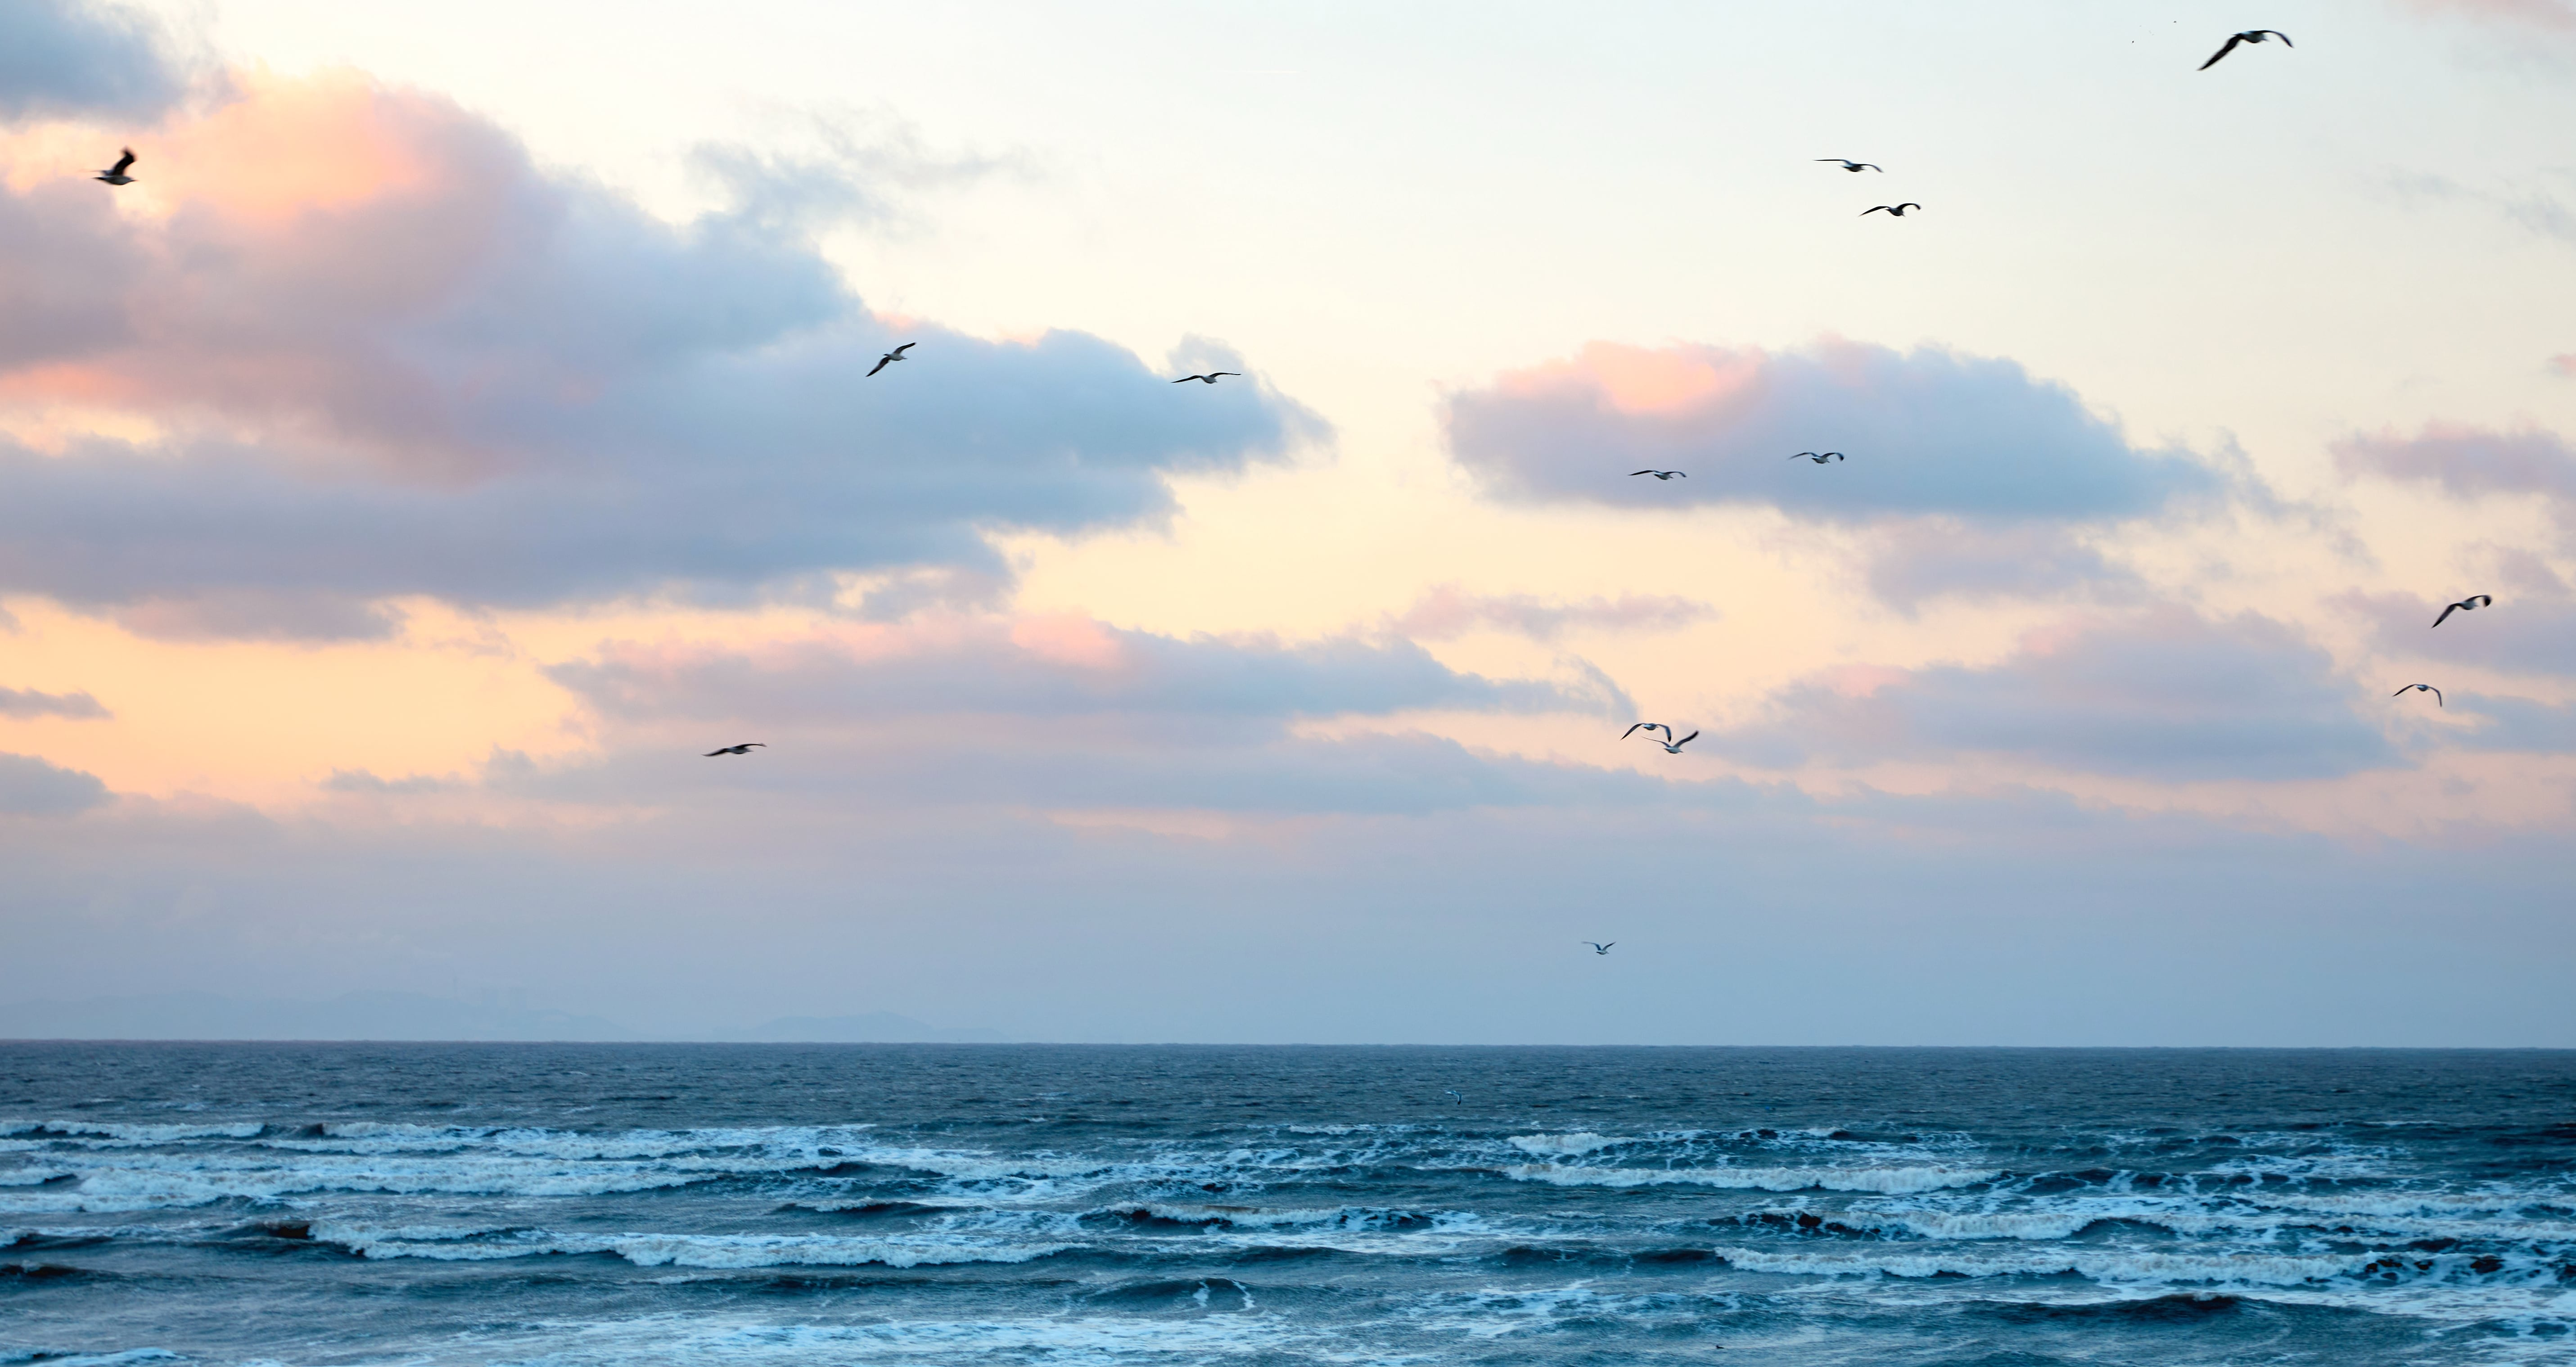
\includegraphics[width=0.75\linewidth]{figures/example2.jpg} % 图片路径
    \caption*{烟台的海、云朵与海鸥。} % 图片说明文字
    \caption{示例图片} % 图片标题
    \label{fig:example1} % 图片标签
\end{figure}
\vspace{-0.7em}  % 减少图片与正文间的间距

\section{代码}
\begin{figure}[H] % 图片位置固定
    \centering % 图片居中
    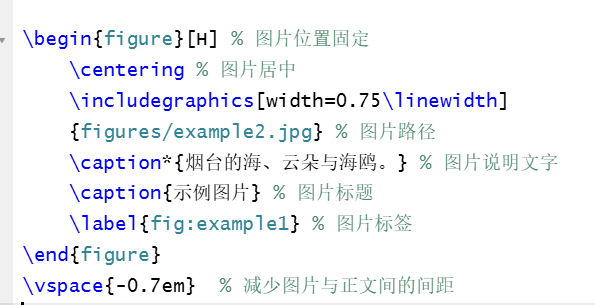
\includegraphics[width=0.75\linewidth]{image0.png} % 图片路径
    \caption*{图片代码} % 图片说明文字
    \caption{} % 图片标题
    \label{fig:example1} % 图片标签
\end{figure}
\vspace{-0.7em}  % 减少图片与正文间的间距

%%%%%%%%%%%%%%%%%%%%%%%%%%%%%%%%%%%%%%%%%%%%%%%%%%%%%%%%%%


\chapter{表格相关}


\section{普通三线表}

在 \LaTeX{} 中,表格的编辑相对较为复杂,推荐使用 Table Generator\footnote{Table Generator 网址:\url{https://www.tablesgenerator.com/}} 来生成表格。为使表格结构更加简洁通用,通常需要使用三线表。三线表是传统网格线表经过简化改造而来的,取消了斜线、竖线和横向分割线,表 \ref{tab:three-line} 是一个三线表的示例。

\begin{table}[H] % 表格位置固定
    \centering % 表格整体居中
    \caption{三线表示例} % 表格表题
    \label{tab:three-line} % 表格标签
    \renewcommand\arraystretch{0.85} % 定义表格行距
    \setlength{\tabcolsep}{12pt} % 定义列间宽度
    \begin{tabular}{ccc} % 表格列样式定义
        \toprule[1.5pt] % 顶线
        \textbf{列名1} & \textbf{列名2} & \textbf{列名3} \\ % 表头
        \midrule[0.8pt] % 栏目线
            Jinan & Jinan & Jinan \\ % 表体
            Yantai & Yantai & Yantai \\ % 表体
            Qingdao &  Qingdao &  Qingdao \\ % 表体
        \bottomrule[1.5pt] % 底线
    \end{tabular}
\end{table}
\vspace{-0.5em}  % 减少表格与正文间的间距

表格如果有附注,尤其是需要在表格中进行标注时,可以使用 \pkg{threeparttable} 宏包。使用的效果如表 \ref{tab:three-line-with-note} 所示。

\begin{table}[H]
    \centering
    \caption{带附注的三线表示例}
    \label{tab:three-line-with-note}
    \renewcommand\arraystretch{0.85} % 定义表格行距
    \setlength{\tabcolsep}{15pt} % 定义列间宽度
    \begin{threeparttable}[c]
        \begin{tabular}{cc}
            \toprule[1.5pt]
            \textbf{山东省}  & \textbf{特色美食}\\
            \midrule[0.8pt]
            烟台           & 鲅鱼水饺、烟台焖子\\
            济南\tnote{a}  & 九转大肠\\
            青岛           & 青岛锅贴、青岛啤酒\\
            威海           & 手撕鲅鱼\\
            \bottomrule[1.5pt]
        \end{tabular}
        \begin{tablenotes}
            %\item [a] {\zihao{5}众所周知,山东济南,中国青岛(狗头)}
        \end{tablenotes}
    \end{threeparttable}
\end{table}
\vspace{-0.9em}  % 减少表格与正文间的间距

\section{长表格}

如某个表需要转页接排,可以使用 longtable 宏包,需要在随后的各页上重复表的编号。
编号后跟表题(可省略)和“(续)”,置于表上方。续表均应重复表头。如表 \ref{tab:longTable} 所示。不过当一个张表内容过多时,建议将该表置于附录中。


\renewcommand\arraystretch{0.85} % 定义表格行距,注意命令的位置与普通表格不同
\begin{longtable}{cccccccc}
    \caption{跨页长表格} \\ % 换页前标题
    
    \toprule[1.5pt]
        \textbf{烟台} & \textbf{长沙} & \textbf{南昌} & \textbf{婺源} & \textbf{天津} & \textbf{上海} & \textbf{北京} & \textbf{青岛} \\ % 换页前表头
    \midrule[0.75pt]
    \endfirsthead
    
    \caption[]{跨页长表格(续)} \\ % 换页后标题
    \toprule[1.5pt]
        \textbf{烟台} & \textbf{长沙} & \textbf{南昌} & \textbf{婺源} & \textbf{天津} & \textbf{上海} & \textbf{北京} & \textbf{青岛} \\  % 换页后表头
    \midrule[0.75pt]
    \endhead
        \bottomrule[1.5pt]
        % \multicolumn{7}{r}{\textit{\zihao{5} \songti 接下页}} \\ 
    \endfoot 
    \bottomrule[1.5pt]
    \endlastfoot
    \label{tab:longTable}
        Row 01 & 01-01 & 01-02 & 01-03 & 01-04 & 01-05 & 01-06 & 01-07 \\
        Row 02 & 02-01 & 02-02 & 02-03 & 02-04 & 02-05 & 02-06 & 02-07 \\
        Row 03 & 03-01 & 03-02 & 03-03 & 03-04 & 03-05 & 03-06 & 03-07 \\
        Row 04 & 04-01 & 04-02 & 04-03 & 04-04 & 04-05 & 04-06 & 04-07 \\
        Row 05 & 05-01 & 05-02 & 05-03 & 05-04 & 05-05 & 05-06 & 05-07 \\
        Row 06 & 06-01 & 06-02 & 06-03 & 06-04 & 06-05 & 06-06 & 06-07 \\
        Row 07 & 07-01 & 07-02 & 07-03 & 07-04 & 07-05 & 07-06 & 07-07 \\
        Row 08 & 08-01 & 08-02 & 08-03 & 08-04 & 08-05 & 08-06 & 08-07 \\
        Row 09 & 09-01 & 09-02 & 09-03 & 09-04 & 09-05 & 09-06 & 09-07 \\
        Row 10 & 10-01 & 10-02 & 10-03 & 10-04 & 10-05 & 10-06 & 10-07 \\
        Row 11 & 11-01 & 11-02 & 11-03 & 11-04 & 11-05 & 11-06 & 11-07 \\
\end{longtable}
\vspace{-0.5em}  % 减少表格与正文间的间距

%%%%%%%%%%%%%%%%%%%%%%%%%%%%%%%%%%%%%%%%%%%%%%%%%%%%%%%%%%

\chapter{版本控制Git}

\section{基础操作}

git help <command> 获取git命令的帮助信息

\begin{figure}[H] % 图片位置固定
    \centering % 图片居中
    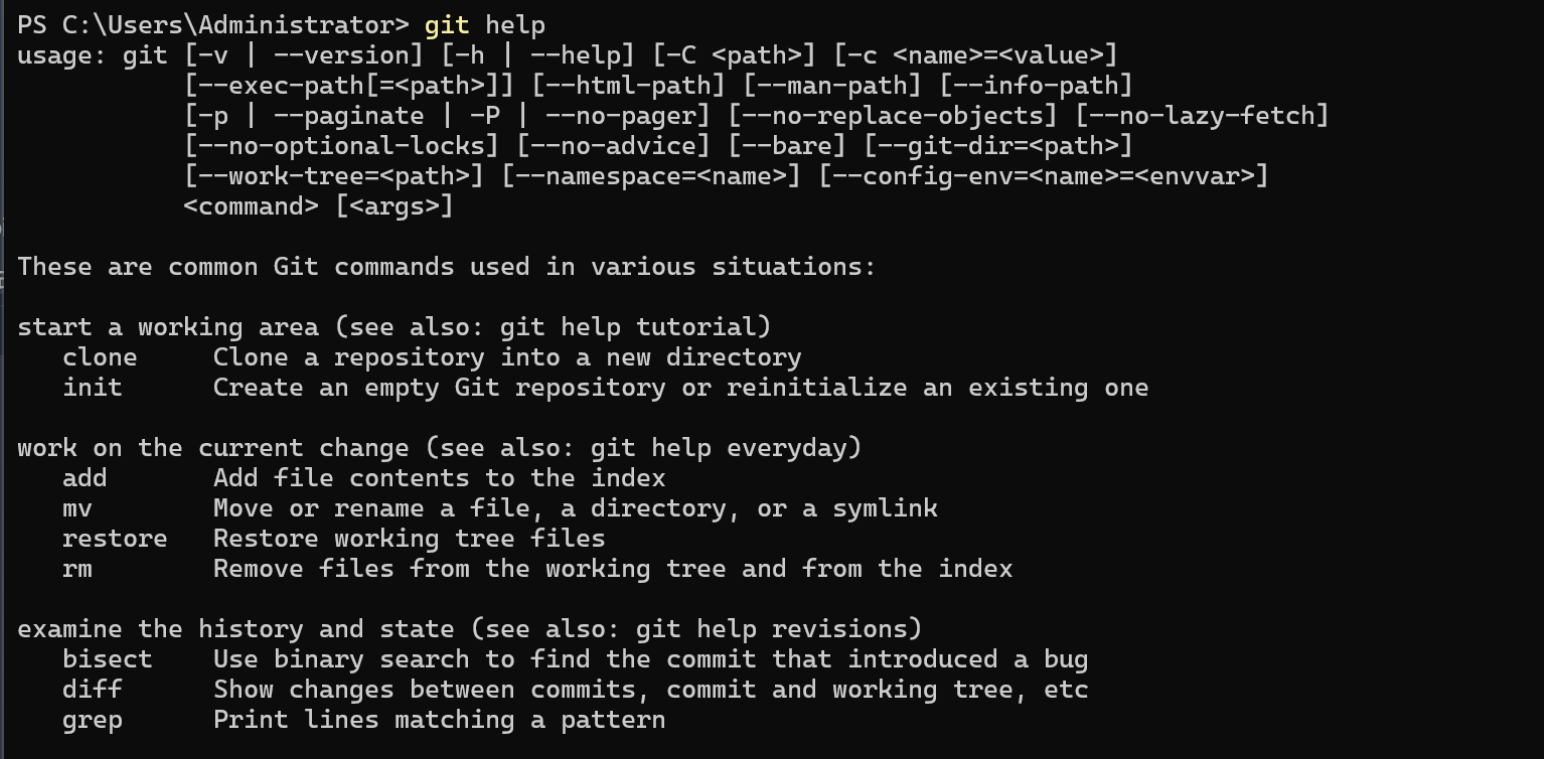
\includegraphics[width=0.9\linewidth]{image1.png}
    \caption*{git help命令图片} % 图片说明文字
    \caption{} % 图片标题
    \label{fig:example1} % 图片标签
\end{figure}
\vspace{-0.7em}  % 减少图片与正文间的间距

使用cd命令进入test文件夹\\

先在github上面将missing-semester-cn.github.io去fork到自己的repositories中,将fork后的repository git clone到test中

\begin{figure}[H] % 图片位置固定
    \centering % 图片居中
    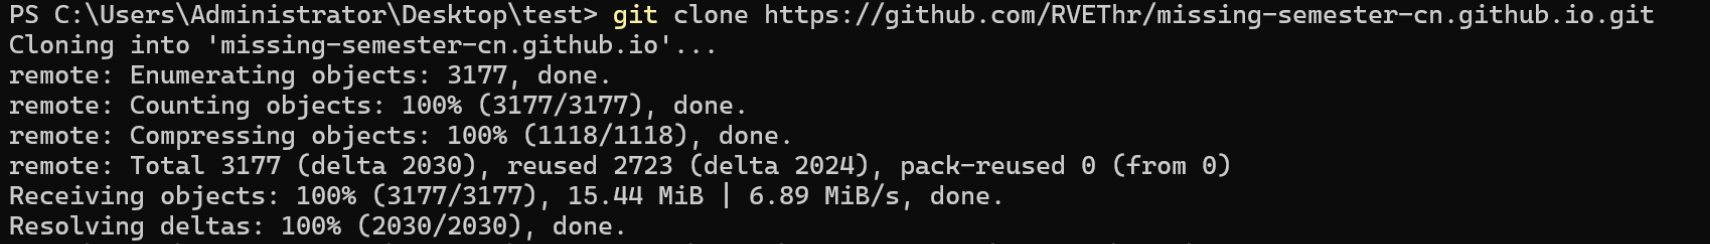
\includegraphics[width=0.9\linewidth]{image2.png}
    \caption*{git clone命令图片} % 图片说明文字
    \caption{} % 图片标题
    \label{fig:example1} % 图片标签
\end{figure}
\vspace{-0.7em}  % 减少图片与正文间的间距

进入刚才clone的仓库,使用git status命令显示当前仓库状态

\begin{figure}[H] % 图片位置固定
    \centering % 图片居中
    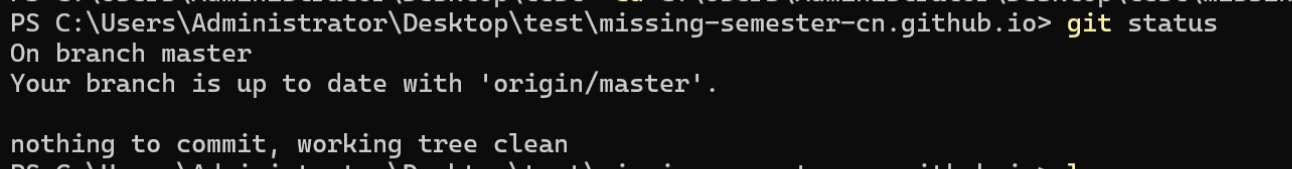
\includegraphics[width=0.9\linewidth]{image3.png}
    \caption*{git status命令图片} % 图片说明文字
    \caption{} % 图片标题
    \label{fig:example1} % 图片标签
\end{figure}
\vspace{-0.7em}  % 减少图片与正文间的间距

创建一个OUC.txt文件,可以使用ls查看文件夹目录,可以看到创建的OUC.txt文件已经在目录中了。

\begin{figure}[H] % 图片位置固定
    \centering % 图片居中
    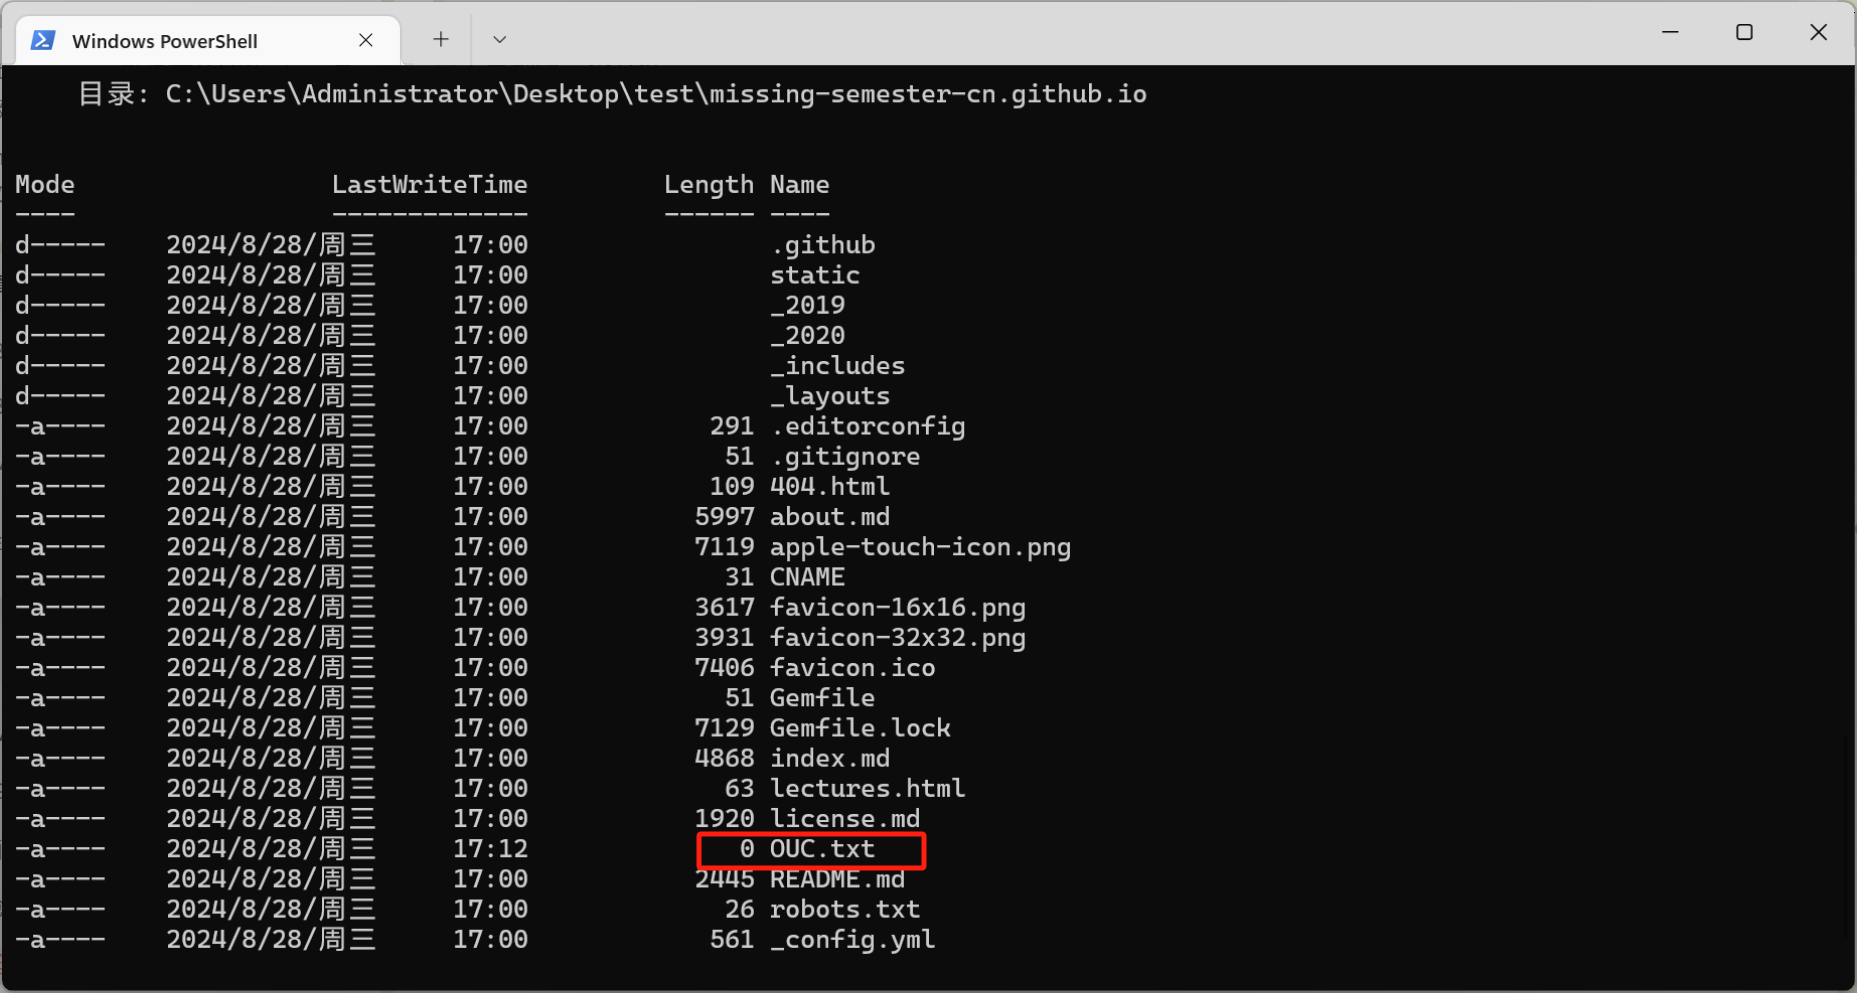
\includegraphics[width=0.9\linewidth]{image4.png}
    \caption*{ls命令图片} % 图片说明文字
    \caption{} % 图片标题
    \label{fig:example1} % 图片标签
\end{figure}
\vspace{-0.7em}  % 减少图片与正文间的间距

将新创建的OUC.txt还没有交给git管理,接下来我们需要使用命令git add将其添加到库中\\
在确认我们提交的文件交由git管理,使用git commit命令\\
(也可以使用git commit -m "提交信息(实例)"来确认并提交信息)

\begin{figure}[H] % 图片位置固定
    \centering % 图片居中
    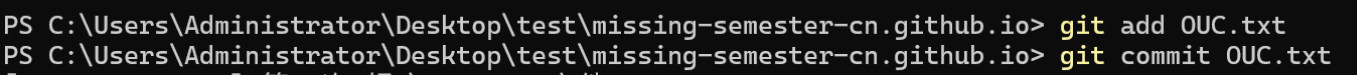
\includegraphics[width=0.9\linewidth]{image5.png}
    \caption*{git add和git commit命令图片} % 图片说明文字
    \caption{} % 图片标题
    \label{fig:example1} % 图片标签
\end{figure}
\vspace{-0.7em}  % 减少图片与正文间的间距

输入后进入如下界面,通过阅读提示可以得知需要我们写入提交信息,输入i进入编辑模式,并在写完后按Esc键后输入:wq回车退出,这个时候我们新创建的OUC.txt文件就被交给了git管理

\begin{figure}[H] % 图片位置固定
    \centering % 图片居中
    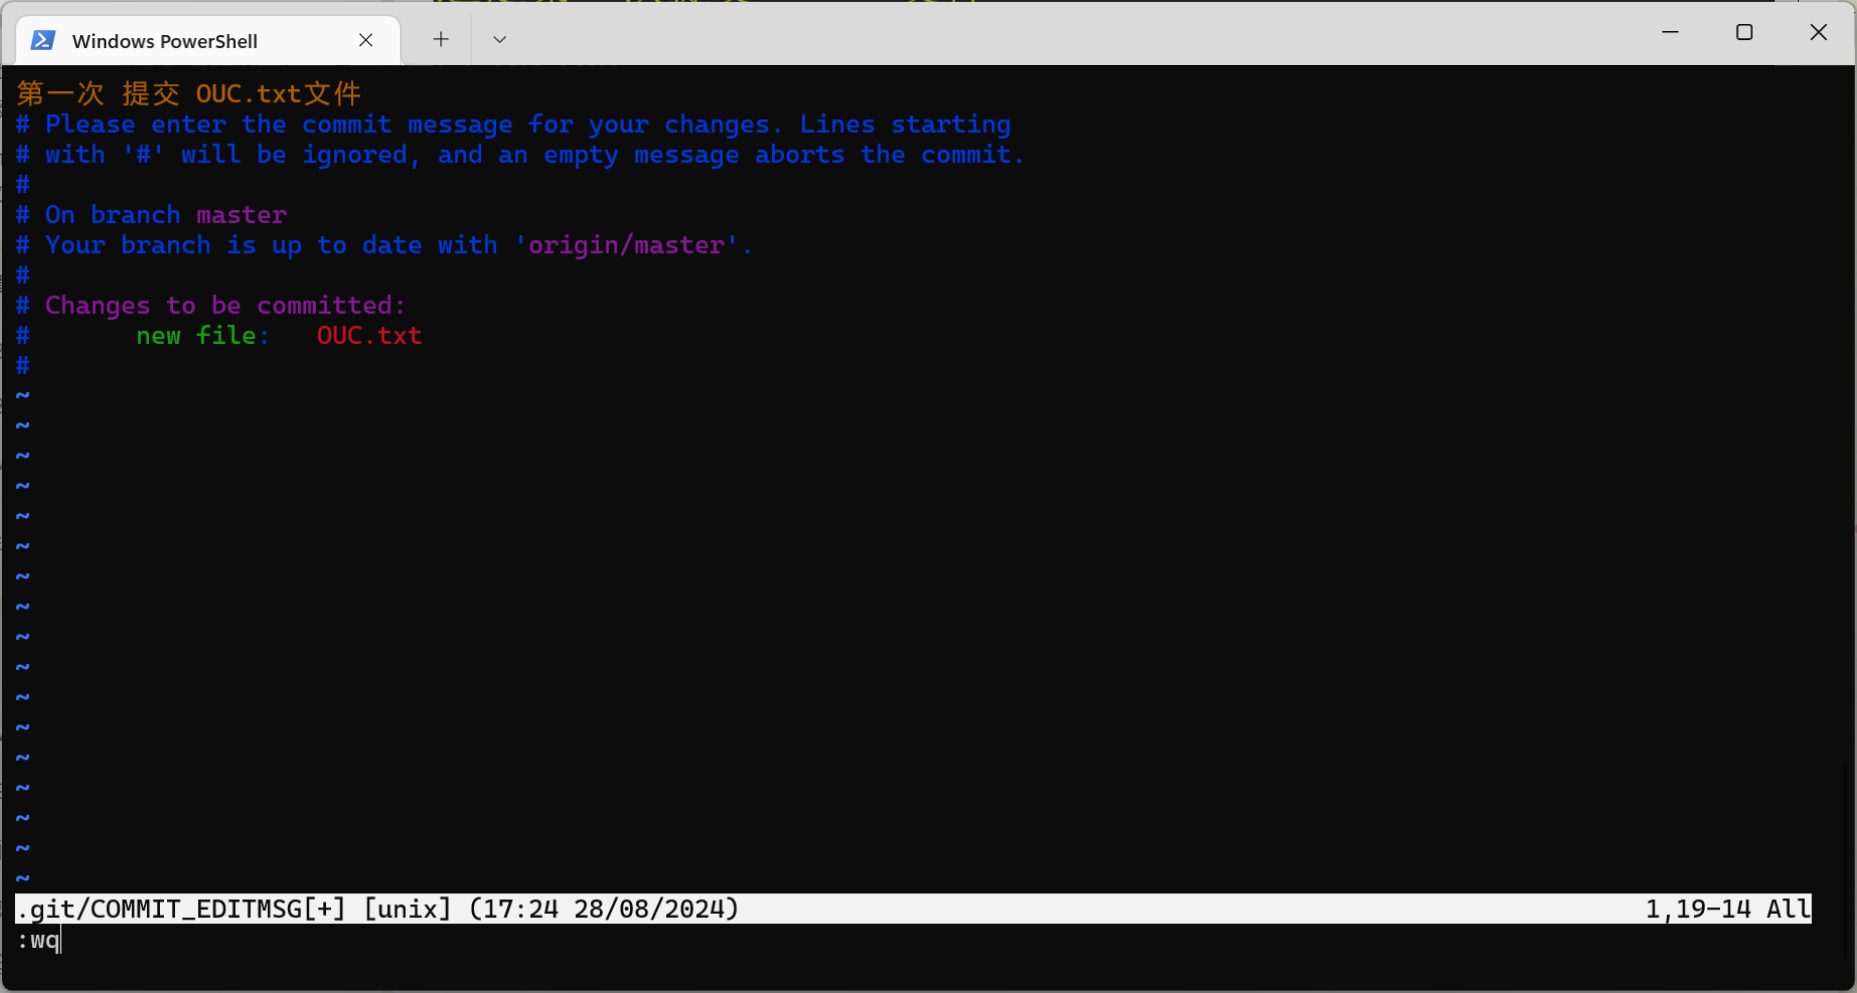
\includegraphics[width=0.6\linewidth]{image6.png}
    %\caption*{} % 图片说明文字
    \caption{} % 图片标题
    \label{fig:example1} % 图片标签
\end{figure}
\vspace{-0.7em}  % 减少图片与正文间的间距

我们对OUC.txt进行一次修改编辑,再使用git status查看会发现如下界面

\begin{figure}[H] % 图片位置固定
    \centering % 图片居中
    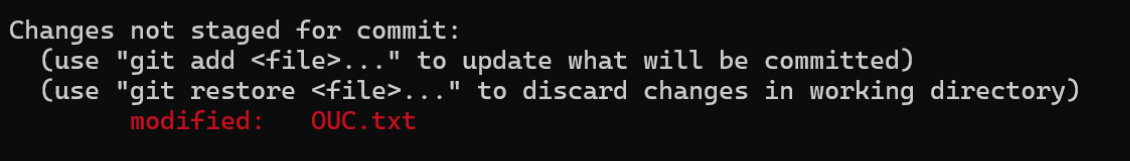
\includegraphics[width=0.9\linewidth]{image7.png}
    %\caption*{} % 图片说明文字
    \caption{} % 图片标题
    \label{fig:example1} % 图片标签
\end{figure}
\vspace{-0.7em}  % 减少图片与正文间的间距

\red{modified: OUC.txt}表示我们的文件被修改了\\

现在我们再add后再看一下仓库的状态

\begin{figure}[H] % 图片位置固定
    \centering % 图片居中
    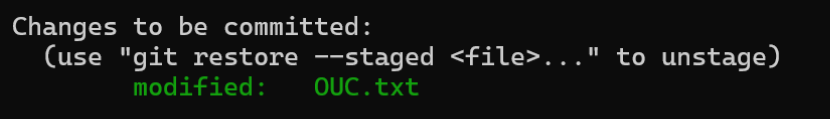
\includegraphics[width=0.9\linewidth]{image8.png}
    %\caption*{} % 图片说明文字
    \caption{} % 图片标题
    \label{fig:example1} % 图片标签
\end{figure}
\vspace{-0.7em}  % 减少图片与正文间的间距

现在是\green{modified: OUC.txt}表示已经添加到版本库中了,接下来我们再提交一下git commit

\begin{figure}[H] % 图片位置固定
    \centering % 图片居中
    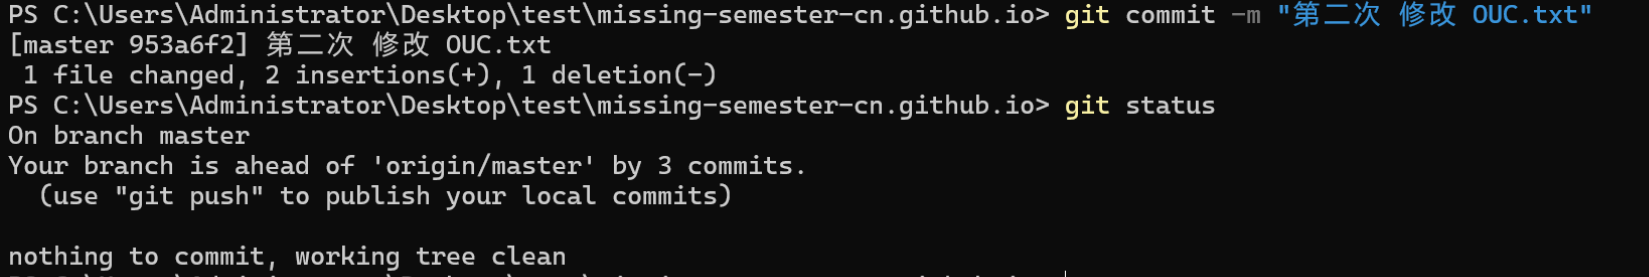
\includegraphics[width=0.9\linewidth]{image9.png}
    %\caption*{} % 图片说明文字
    \caption{} % 图片标题
    \label{fig:example1} % 图片标签
\end{figure}
\vspace{-0.7em}  % 减少图片与正文间的间距

现在可以看到状态回到最初的nothing to commit, working tree clean,说明我们修改的文件确实被提交上了。\\

到此为止我们的文件已经改到了第三版了,可以使用git log来查看git的历史记录

\begin{figure}[H] % 图片位置固定
    \centering % 图片居中
    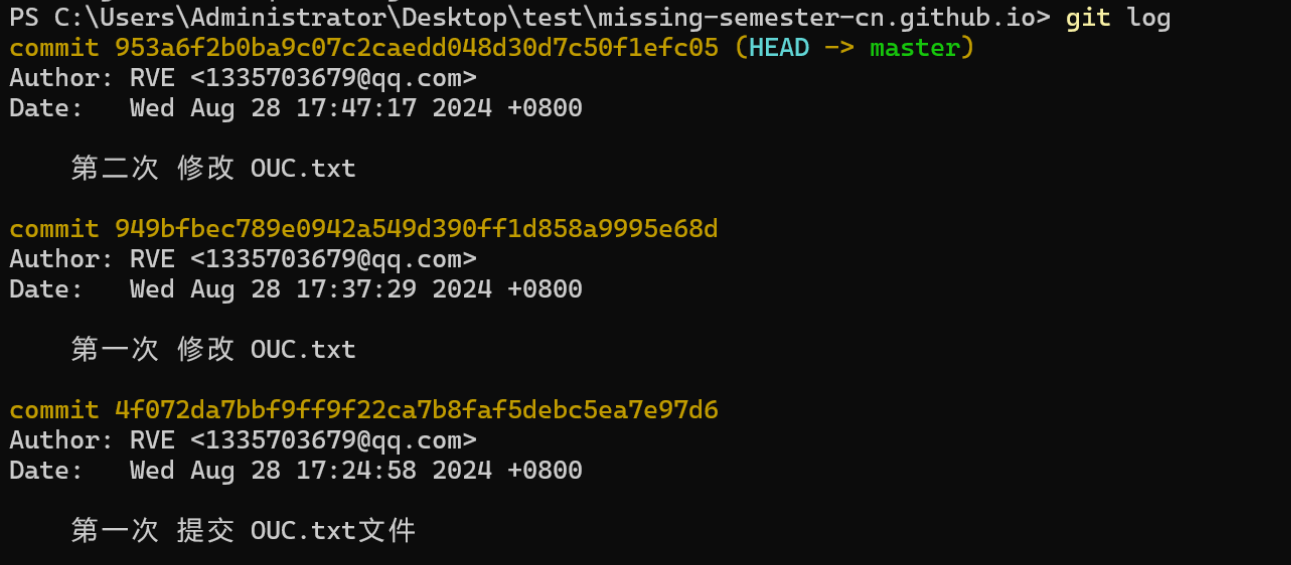
\includegraphics[width=0.9\linewidth]{image10.png}
    \caption*{git log命令图片} % 图片说明文字
    \caption{} % 图片标题
    \label{fig:example1} % 图片标签
\end{figure}
\vspace{-0.7em}  % 减少图片与正文间的间距

如果我们想要回退版本可以使用指令git reset --hard 版本号的方式来进行,如下图所示:

\begin{figure}[H] % 图片位置固定
    \centering % 图片居中
    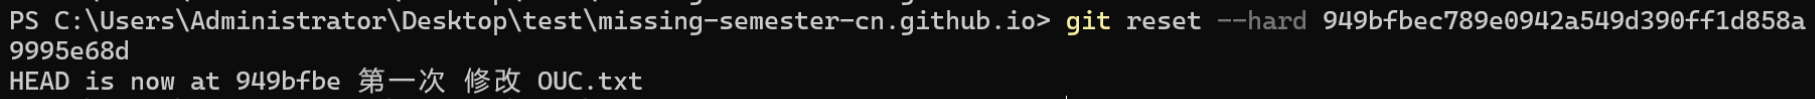
\includegraphics[width=0.9\linewidth]{image11.png}
    \caption*{git reset --hard回退版本命令图片} % 图片说明文字
    \caption{} % 图片标题
    \label{fig:example1} % 图片标签
\end{figure}
\vspace{-0.7em}  % 减少图片与正文间的间距


可以看到我们现在已经回退到了第一次修改的版本了\\
如果要回到回退前的版本,也可以使用git reset --hard的命令来进行,如下图:

\begin{figure}[H] % 图片位置固定
    \centering % 图片居中
    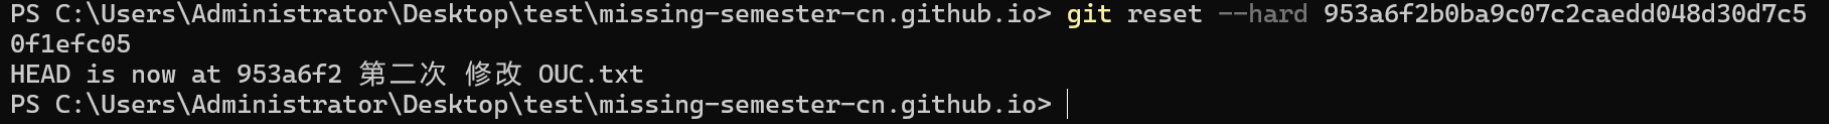
\includegraphics[width=0.5\linewidth]{image12.png}
    \caption*{回退之前版本命令图片} % 图片说明文字
    \caption{} % 图片标题
    \label{fig:example1} % 图片标签
\end{figure}
\vspace{-0.7em}  % 减少图片与正文间的间距

将我们对本地仓库的更改推送到远程仓库使用git push命令来完成同步本地提交到远程版本控制系统。

\begin{figure}[H] % 图片位置固定
    \centering % 图片居中
    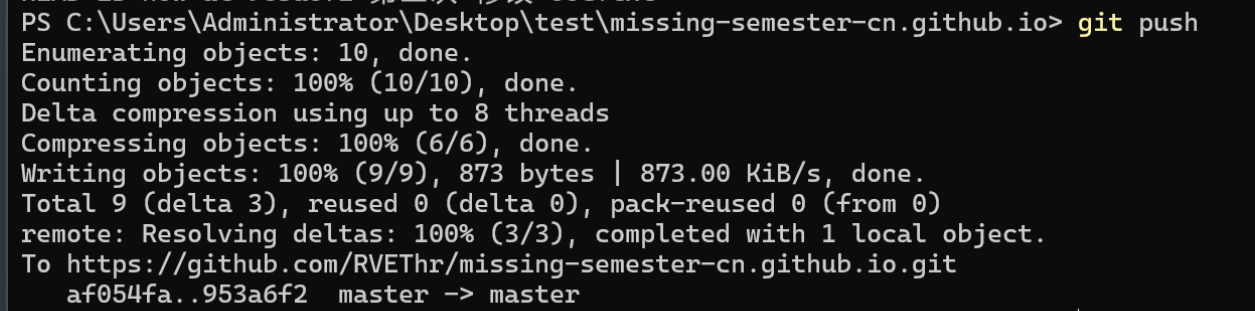
\includegraphics[width=0.9\linewidth]{image13.png}
    \caption*{git push命令图片} % 图片说明文字
    \caption{} % 图片标题
    \label{fig:example1} % 图片标签
\end{figure}
\vspace{-0.7em}  % 减少图片与正文间的间距

\begin{figure}[H] % 图片位置固定
    \centering % 图片居中
    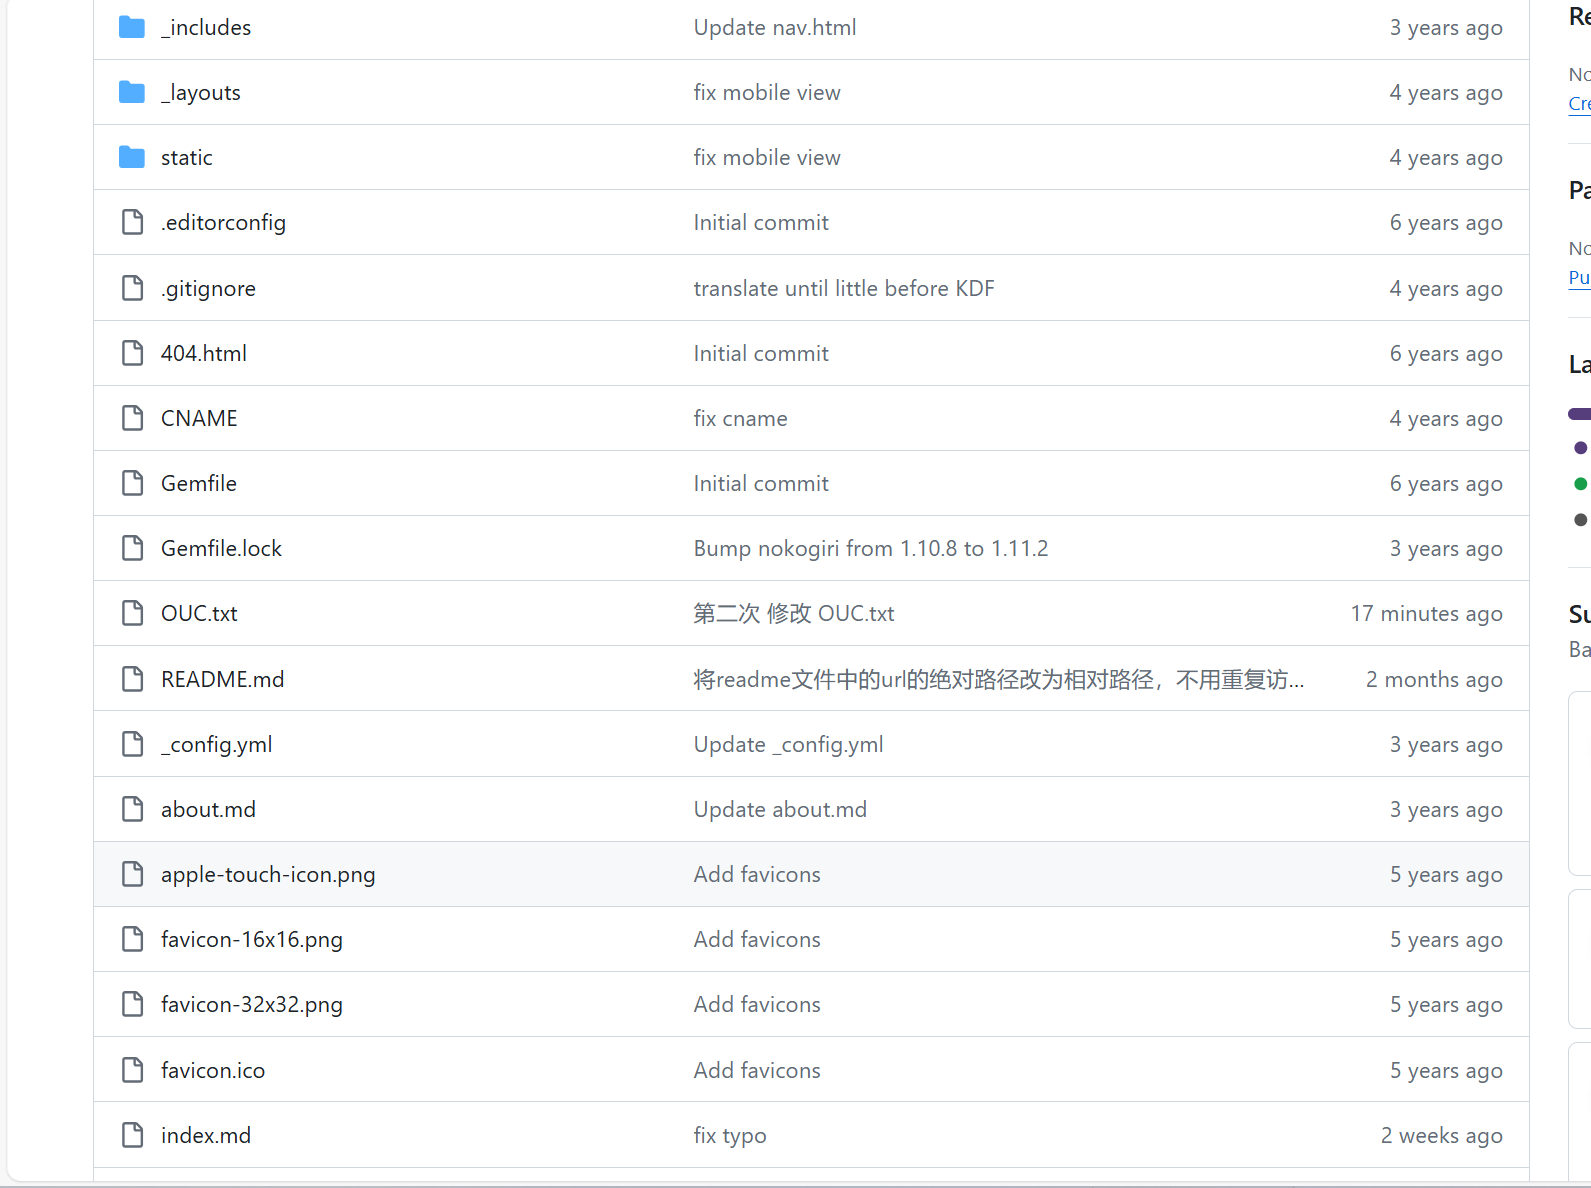
\includegraphics[width=0.9\linewidth]{image14.png}
    \caption*{github上传成功图片} % 图片说明文字
    \caption{} % 图片标题
    \label{fig:example1} % 图片标签
\end{figure}
\vspace{-0.7em}  % 减少图片与正文间的间距

还有一种命令git pull是与git push不同的,git pull是用于从远程仓库获取最新更改并合并到当前分支的命令,如果出现冲突,Git 会提示你手动解决冲突。

解题感悟:\\
在这次版本控制(Git)和LaTeX文档编辑的实验中,我深刻地体会到了工具的重要性以及它们在学术和工作中的应用价值。\\

首先,通过使用Git进行版本控制,我体会到了管理代码和文档的便捷性。Git的分支和合并功能让我在多个项目版本之间自由切换,而不必担心丢失进度或数据。每次提交(commit)都能精确地记录下我所做的更改,使我能够轻松回溯到任何历史版本。这种对版本历史的掌控感让我在实验过程中更加自信,同时也认识到在团队协作中,Git能大大减少冲突和重复劳动。\\

在使用LaTeX进行文档编辑时,我感受到了它在排版上的强大功能,尤其是在处理复杂的数学公式和图表时,LaTeX的优势非常明显。虽然LaTeX的语法相对其他文档编辑器更为复杂,但它带来的文档精确控制和专业排版效果,使得学习和使用它是非常值得的。通过实验,我不仅掌握了LaTeX的基本语法,还学会了如何利用模板和宏命令来提高工作效率。\\

这次实践过程让我对Git和LaTeX有了更加深入的了解,也让我认识到,在日后的学习和科研工作中,这两项技能将是不可或缺的工具。Git能帮助我高效管理代码和文档,而LaTeX则能让我更专业地呈现学术成果。\\

此次报告的github链接:


%%%%%%%%%%%%%%%%%%%%%%%%  参考文献  %%%%%%%%%%%%%%%%%%%%%%%%

\begin{references}
    \bibliography{references.bib} % 指定.bib文件路径
\end{references}

%%%%%%%%%%%%%%%%%%%%%%%%%  附录  %%%%%%%%%%%%%%%%%%%%%%%%%%

\StartAppendix % 启用附录

\chapter{附录}

附录

%%%%%%%%%%%%%%%%%%%%%%%  正文后页眉  %%%%%%%%%%%%%%%%%%%%%%

% 页眉(关闭页眉务必将页眉类型设为empty)
\Header
    {common} % 页眉类型:common、publish、empty
    {1pt} % 上分隔线宽度
    {1pt} % 两线距离
    {0.5pt} % 下分割线宽度
    {} % 页眉左自定义内容(文本或图片)
    {
\includegraphics[width=0.25\textwidth]{figures/logos/HNU-title-EN.png}} % 页眉中自定义内容(文本或图片)
    {} % 页眉右自定义内容(文本或图片)

%============================================%

% 页脚(关闭页脚务必将页脚类型设为empty) 
\Footer
    {common} % 页脚类型:common、publish、empty
    {0pt} % 上分隔线宽度
    {0pt} % 两线距离
    {0pt} % 下分割线宽度
    {} % 页脚左自定义内容(文本或图片)
    {\thepage} % 页脚中自定义内容(文本或图片)
    {} % 页脚右自定义内容(文本或图片)

%============================================%

% 页数样式 参数:#1起始页数
% \setRomanPageNumber{1} % 设置罗马数字页码
% \setArabicPageNumber{1} % 设置阿拉伯数字页码

%%%%%%%%%%%%%%%%%%%%%%%%%  致谢  %%%%%%%%%%%%%%%%%%%%%%%%%

%\StartAcknowledgements % 启用致谢

\end{document}